
\chapter{Contextualizaci\'on}

\todo[inline]{INTRO AL CAPITULO!, explicando los temas variados!}

% ================================================================
% ================================================================
% ================================================================

\section{Robots de servicio}

La Federaci\'on Internacional de Rob\'otica (IFR)\cite{IFR} define \textit{robot} como:
\begin{quotation}
``Un mecanismo actuado y programable en dos o m\'as ejes y con un cierto grado de autonom\'ia, que se mueve en su entorno para realizar tareas previstas. En este contexto, autonom\'ia se refiere a la habilidad de realizar tareas previstas, basado en el estado actual y lo sensado, sin intervenci\'on humana.''
\end{quotation}

Asimismo, la IFR define un \textit{robot de servicio} como un robot ``que realiza tareas \'utiles para humanos o equipamiento, excluyendo aplicaciones de automatizaci\'on industrial''. As\'i, un robot de servicio debe trabajar en ambientes no controlados y con la autonom\'ia suficiente que le permita llevar a cabo su cometido. Generalmente, la rob\'otica de servicio se enfoca en asistir a los seres humanos en tareas repetitivas y comunes.

Seg\'un su \'area de aplicaci\'on, un rob\'ot de servicio se clasifica en \textit{de uso personal} o \textit{de uso profesional}. Los primeros son utilizados en ambientes no comerciales y por personas comunes; como por ejemplo, un robot sirviente o una silla de ruedas aut\'onoma. Un robot de servicio profesional se utiliza en ambientes comerciales, usualmente operados por alguien entrenado; un ejemplo son los robots de entrega de paquetes o para cirug\'ia.


\subsection{Robots Dom\'esticos}\label{sec:domestic_robots}

Seg\'un la recopilaci\'on de datos realizada por la IFR durante el 2016, este tipo de robots es utilizado en las siguientes \'areas:
\begin{itemize}[topsep=0pt]
\setlength\itemsep{0.2em}
\item Tareas dom\'esticas: De compa\~nia, asistencia, limpieza, cuidado del hogar.
\item Entretenimiento: Juguetes, comunicaci\'on, educaci\'on e investigaci\'on.
\item Asistencia a ancianos y discapacitados: Sillas rob\'oticas y robots para cuidar personas.
\item Transporte.
\item Seguridad y vigilancia.
\item Otros que no caen en las categor\'ias anteriores.
\end{itemize}
\bigskip

El foco de este trabajo son los robots de servicio personales, dedicados a tareas dom\'esticas, clasificaci\'on a la que en  adelante se referir\'a como \textit{Robots Dom\'esticos}.

Para entender el alcance del trabajo, en cuanto a qu\'e es lo que se espera del sistema, a continuaci\'on se listan algunas capacidades de los robots dom\'esticos. Un robot de compa\~nia y asistencia tiene, pero no se limita a las siguientes tareas:
\begin{itemize}[topsep=0pt]
\setlength\itemsep{0.2em}
\item Interacci\'on amistosa con humanos.
\item Ayudar a recordar y organizar tareas.
\item Cooperar con la realizaci\'on de un procedimiento.
\item Guiar y seguir a personas.
\item Recordar informaci\'on y entidades.
\end{itemize}
\bigskip

Algunas tareas que robots dom\'esticos de tipo mayordomo deben ejecutar son:
\begin{itemize}[topsep=0pt]
\setlength\itemsep{0.2em}
\item Ofrecer comida y bebestibles.
\item Preparaci\'on de comida.
\item Ordenar y limpiar el hogar.
\end{itemize}
\bigskip

% ================================================================
% ================================================================
% ================================================================

\section{Memoria Humana}

\todo[inline]{Faltan varias referencias!... ver... referencias a psicoanalisis \cite{Deutsch2008} }


La memoria es un elemento fundamental para los humanos en su d\'ia a d\'ia, es parte integral de su existencia. P ermite recordar qui\'en, qu\'e, c\'omo, d\'onde y cu\'ando. En t\'erminos psicol\'ogicos, es la habilidad para para codificar, almacenar y luego obtener informaci\'on sobre eventos pasados, en el cerebro. Los pensamientos son parte de la memoria de corto plazo, mientras que eventos pasados son almacenados en una memoria de largo plazo. Existen muchos estudios en el \'area de la psicolog\'ia cognitiva con diversas descripciones y modelos te\'oricos de cada tipo de memoria\cite{Vijayakumar2014}.

Desde el punto de vista de la informaci\'on procesada, la memoria es vista como una facultad humana consistente en procesos para el manejo de informaci\'on. Los 3 componentes principales son:

\begin{itemize}
\item Codificaci\'on: En este paso, se adquiere nueva informaci\'on desde los sentidos humanos. Los datos son convertidos a un formato que pueda ser almacenado en la estructura cerebral correspondiente.
\item Almacenamiento: Consiste en la creaci\'on de registros permanentes de informaci\'on. Es un proceso pasivo, de continuo procesamiento para clasificar datos nuevos y los ya existentes en el cerebro.
\item Adquisici\'on: Hace referencia al acceso de datos almacenados. El proceso se realiza en el momento, para obtener una reconstrucci\'on aproximada de la informaci\'on, a partir de elementos repartidos en distintas partes del cerebro.
\end{itemize}


La memoria puede ser dividida en m\'ultiples sistemas de independientes, con funcionalidades bien definidas y sustentados por distintas estructuras cerebrales. La primera diferenciaci\'on define dos tipos de memoria: la memoria de corto y la de largo plazo, STM (Short-Term Memory) y LTM (Long-Term Memory), por sus siglas en ingl\'es. En el diagrama de la figura \ref{img:human_memory} se muestra una separaci\'on cl\'asica utilizada en el \'area de las ciencias cognitivas\cite{Eichenbaum:2008}, explicada en las siguientes subsecciones.

\begin{figure}[H]
\centering
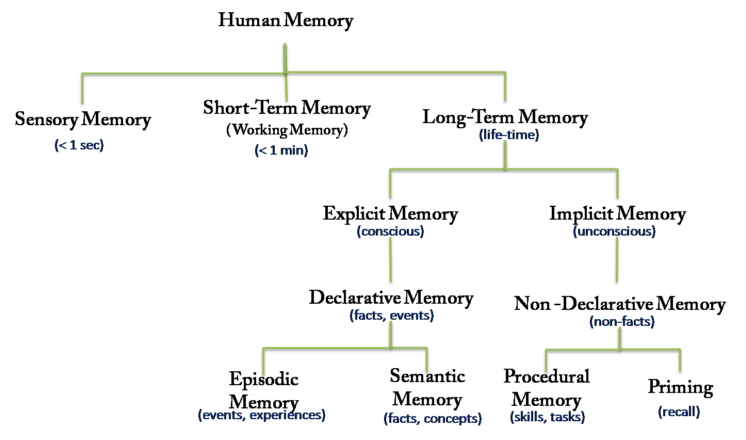
\includegraphics[width=0.8\textwidth]{./figures/diagrama_memoria.png}
\caption{\small Clasificaciones de la memoria humana. Obtenido de \cite{Vijayakumar2014}.}
\label{img:human_memory}
\end{figure}

% Sobre el estudio de la memoria.. origenes.. Tulving 

\subsection{Memoria de Corto Plazo}

En el \'ambito cognitivo, la STM se refiere a la habilidad de estar atento, recopilar informaci\'on  y memorias, para luego utilizarlas dentro de un corto periodo de tiempo. Es responsable de almacenar informaci\'on constantemente y de decidir que parte ser\'a transferida a la memoria de largo plazo. El t\'ermino de \textit{Memoria de Trabajo} suele ser utilizado de manera intercambiable con el de STM. Adem\'as, suele ser agrupada con otro tipo de memoria, llamada \textit{Sensorial}.

La STM se caracteriza por manejar informaci\'on muy detallada, ser de poca capacidad y permitir un r\'apido acceso a estos datos. Permite recordar r\'apidamente y con gran detalle experiencias ocurridas hace pocos segundos, pero con dificultad creciente a medida que avanza el tiempo.

Se sustenta principalmente en la corteza prefrontal del cerebro. Algunos estudios han mostrado que las neuronas involucradas son capaces de mantener informaci\'on relevante de corto plazo, la que es combinada con informaci\'on sensorial entrante y \'areas que manejan la toma de decisiones. %(Miller, 2000).
En los humanos esta \'area presenta gran activaci\'on durante procesos de codificaci\'on, acceso y manipulaci\'on de memorias. %(Postle, 2006). 


\subsection{Memoria de Largo Plazo}

La LTM se asocia al almacenamiento permanente de informaci\'on en el cerebro. Se caracteriza por manejar mucha informaci\'on sobre experiencias y entidades, ser menos detallada y proveer un acceso m\'as lento a los recuerdos, respecto a la STM\cite{Eichenbaum:2008}. Cierta informaci\'on de la STM eventualmente es transferida a la LTM. De acuerdo a la figura \ref{img:human_memory}, sus dos principales categor\'ias son la \textit{Memoria Impl\'icita} y la \textit{Memoria Expl\'icita}.
% algunos creen que no est\'a limitada en su capacidad de almacenar informaci\'on.

\subsubsection{Memoria Impl\'icita}

La memoria impl\'icita  abarca la capacidad de aprender habilidades, h\'abitos y preferencias, caracterizados por ser mejorados o adquiridos sin una recolecci\'on consciente. As\'i, tambi\'en suele ser denominada \textit{memoria inconsciente} o \textit{memoria no declarativa}, pues comprende acciones que pueden ser realizadas sin pensar en ellas. Ejemplos de esto, son el andar en bicicleta o tocar un instrumento musical.

Se puede clasificar en \textit{memoria procedural} (P-LTM) y en \textit{memoria de primado}. La primera ayuda a realizar tareas sin pensar en ellas, es decir, maneja el conocimiento del \textit{C\'omo}; Ejemplos de esto son comer y caminar. La memoria de primado hace referencia a la predisposici\'on para recordar hechos o informaci\'on a la que un sujeto es expuesto con anterioridad; Ejemplos de esto son la facilidad para recordar canciones escuchadas hace poco tiempo, o el uso de palabras e ideas vistas recientemente.

Se ha mostrado que la P-LTM se sustenta en el cerebelo, mediante la activaci\'on de este durante el uso de habilidades motoras.

Otro tipo de memoria implic\'ita es la \textit{memoria emocional} (Em-LTM). Se encarga de dar significado afectivo a ciertos  est\'imulos, que de otra forma ser\'ian neutrales. Las estructuras cerebrales involucradas son la am\'igdala, \'areas corticales y subcorticales. Esta memoria se expresa mediante la activaci\'on del hipot\'alamo, en conjunto al sistema nervioso simp\'atico, generando reacciones emocionales y sentimientos.


\subsubsection{Memoria Expl\'icita}

La memoria expl\'icita suele ser denominada \textit{memoria consciente} o \textit{memoria declarativa}, pues maneja conocimientos relacionados a hechos y eventos adquiridos de forma consciente. Seg\'un las estructuras cerebrales involucradas, se conforma de la \textit{memoria epis\'odica} y de la \textit{memoria sem\'antica}.

La memoria epis\'odica (Ep-LTM) es de car\'acter  autobiogr\'afico y almacena detalles de eventos y experiencias pasadas. Permite responder a las preguntas ``Qu\'e sucedi\'o'', ``D\'onde ocurri\'o'' y ``Cu\'ando ocurri\'o''. Un humano puede acceder a esta memoria si es capaz de decir: ``recuerdo que''. Este tipo de memoria da al ser humano la sensaci\'on de continuidad en el tiempo.

La memoria sem\'antica (S-LTM) almacena el conocimiento de hechos, significados, categor\'ias y proposiciones. Un humano puede acceder a esta memoria si es capaz de decir: ``s\'e que''. Esta memoria se abstrae de perspectiva e informaci\'on situacional.

Las estructuras cerebrales que soportan la memoria expl\'icita son el hipocampo, encargado de manejar la Ep-LTM, junto a la corteza cerebral, en donde se distribuyen los conocimientos de la S-LTM. En el hipocampo se mantienen conexiones neuronales a los sectores de inter\'es de la corteza, en donde se alojan conocimientos sem\'anticos asociados a cada episodio.

Un ejemplo de uso de Ep-LTM es el recuerdo de una graduaci\'on escolar, el lugar y la fecha donde ocurri\'o. La S-LTM podr\'ia responder en que consiste una graduaci\'on y describir la ropa que se suele ocupar en ellas.


\subsection{Plasticidad Sin\'aptica y Modulaci\'on}

Se denomina \textit{consolidaci\'on} de memoria al proceso de transici\'on de conocimiento desde la STM a la LTM. Durante la consolidaci\'on se generan conexiones neuronales entre la Ep-LTM y la respectiva zona sem\'antica. Para activar la consolidaci\'on se requiere de un est\'imulo relevante, sumado a la cadena de eventos para el almacenamiento.

Se denomina \textit{deterioro} de memoria u ``olvido'' al proceso de debilitamiento de las conexiones neuronales establecidas por los procesos de consolidaci\'on. Est\'a en constante funcionamiento, degenerando las asociaciones entre la Ep-LTM y la S-LTM. Por lo tanto, en este contexto, el olvido no significa una eliminaci\'on de los datos en el cerebro, sino que estos siguen ah\'i, pero la conexi\'on requerida es inexistente o es demasiado d\'ebil para poder ocuparla.

Existen procesos qu\'imicos a nivel cerebral que afectan la consolidaci\'on y el deterioro de la LTM. Hay evidencia de que estos est\'an en continuo funcionamiento. Estos eventos celulares ocurren en una escala de segundos a minutos, y son esenciales para la mantenci\'on de la memoria a largo plazo.

Es posible modular ambos procesos. Las experiencias repetidas potencian la consolidaci\'on de la memoria, lo que fortalece las conexiones neuronales. Por otro lado, la memoria emocional es capaz de potenciar o deprimir las reacciones qu\'imicas requeridas; seg\'un los est\'imulos a los que se enfrente, modifica el nivel de relevancia de los eventos, pudiendo generar memorias muy fuertes y h\'abitos arraigados. Ejemplos de esto, son la memorizaci\'on por repetici\'on, los flashbacks y las memorias asociadas a eventos importantes como cumplea\~nos.

% ================================================================
% ================================================================
% ================================================================

\section{Memoria y rob\'otica}

En esta secci\'on se presenta el estado del arte respecto al uso de LTM en rob\'otica. En primer lugar se presenta la importancia de la LTM y las expectativas para un robot dom\'estico. Luego se hace una comparaci\'on entre la memoria humana y el manejo de informaci\'on en robots.  Se presenta el estado del arte para cada componente cognitivo de inter\'es. Finalmente, se describen otros enfoques de la literatura para la implementaci\'on de LTMs, que no est\'an basados en el enfoque biol\'ogico utilizado en este proyecto.


\subsection{Relevancia de la memoria rob\'otica}

La memoria es una habilidad esencial para cualquier ser social. Lo mismo aplica para un robot dom\'estico cuya misi\'on sea establecer una relaci\'on de largo plazo con usuarios humanos. Un problema com\'un es que los usuarios tienden a perder el inter\'es r\'apidamente en los robots, debido a la falta de vida y expectativas no cumplidas, respecto a la inteligencia y capacidad de socializar de la m\'aquina. El problema se potencia con el paso del tiempo, donde la motivaci\'on por interactuar disminuye y se genera frustraci\'on, a medida que el robot continua repitiendo los mismos comportamientos predefinidos\cite{Ho2009}.

Si se desea mejorar la interacci\'on humano-robot, entonces se requiere que el robot se comporte de manera m\'as natural. Los mejores agentes rob\'oticos sociales deber\'ian satisfacer las necesidades cognitivas y sociales humanas; mientras m\'as familiar sea la interacci\'on, ser\'an m\'as efectivos en su prop\'osito. As\'i, la LTM es una habilidad crucial si se espera que el robot sea capaz de aprender y adaptarse a su entorno.


Por otro lado, desde un punto de vista pr\'actico, se ha mostrado que el concepto de memoria LTM aplicada a robots es beneficioso. En \cite{Salgado2012} ocupan memoria P-LTM para mejorar el desempe\~no de un robot en ambientes din\'amicos, logrando acelerar el proceso de adaptaci\'on al entorno y la toma de decisiones.

%... blabla util \cite{Vijayakumar2014}


%\subsubsection{Requerimientos para robots dom\'esticos}
%
%En t\'erminos de LTM, un robot dom\'estico necesita poder recordar los siguientes conocimientos:
%
%... \todo[inline]{tareas de un robot de servicio}
%\begin{itemize}
%\item 
%\end{itemize}
%
%... casos de uso e inferencia \cite{Vijayakumar2014}
%
%... artificial companion PAG 13 \cite{Vijayakumar2014}
%


\subsection{Relaci\'on entre memoria humana y memoria rob\'otica}


Son muchos los trabajos en LTM que han basado su desarrollo en la taxonom\'ia de la memoria humana, donde se implementan esquemas de informaci\'on con m\'odulos an\'alogos a los presentados en la figura \ref{img:human_memory}. Esto se puede justificar por la similitud de cada tipo de memoria, con m\'odulos preexistentes en la arquitectura rob\'otica. A continuaci\'on se presenta una comparaci\'on entre cada tipo de memoria y sus procesos, y el an\'alogo rob\'otico.

\subsubsection{Memoria STM}

Se relaciona a todos los datos que est\'an actualmente cargados en la memoria primaria de la m\'aquina. Esta memoria es la utilizada para solucionar la tarea actual, es equivalente a los pensamientos del robot y cumple con las caracter\'isticas de la STM humana: es volátil, de r\'apido acceso y limitada en capacidad. Tambi\'en se encuentra presente en todo archivo temporal manejado por el sistema, mientras est\'a en funcionamiento. As\'i, la estructura equivalente a la cerebral ser\'ia la RAM de la m\'aquina.


\subsubsection{Memoria S-LTM}

La memoria S-LTM es com\'un y se puede asociar a casi toda fuente de datos est\'atica, no utilizada por las otras memorias. Luego, la S-LTM se sustenta en la memoria secundaria, cumpliendo las caracter\'isticas de la LTM humana: es persistente, de acceso costoso y virtualmente ilimitada en capacidad. Algunos ejemplos son:
\begin{itemize}[topsep=0pt]
\setlength\itemsep{0.2em}
\item Bases de datos.
\item Directorios con im\'agenes de personas y objetos conocidos.
\item Mapa con descripci\'on del ambiente.
\item Frases predefinidas que puede decir el robot.
\item Archivos de audio utilizados por el robot.
\item En general, todo archivo con datos persistentes, cargados en cada sesi\'on de trabajo.
\end{itemize}


\subsubsection{Memoria P-LTM}

Este tipo de memoria es comparable a algoritmos predefinidos para realizar acciones, generalmente motoras. 

Algunos ejemplos comparables son: 
\begin{itemize}[topsep=0pt]
\setlength\itemsep{0.2em}
\item Algoritmos basados en redes neuronales, entrenados para manipular objetos o reconocer patrones.
\item Algoritmos entrenados para tareas espec\'ificas, c\'omo la detecci\'on de caras o el reconocimiento de voz.
\item Controladores basados en puntos de operaci\'on para acciones motoras.
\item S\'intesis de voz
\end{itemize}

Las estructuras equivalentes a la versi\'on cerebral ser\'ian los archivos con par\'ametros para cada algoritmo, obtenidos a partir del entrenamiento o ajustados manualmente.


\subsubsection{Otros tipos de memoria}

Generalmente, tanto STM, S-LTM como P-LTM son un requisito m\'inimo para el funcionamiento de un software rob\'otico, por lo que no son implementadas conscientemente. Luego, la existencia de tales memorias, no implica la intenci\'on de crear una arquitectura LTM similar a la humana. Los otros tipos de memorias s\'olo son implementados en casos especializados.



\subsection{Memoria LTM expl\'icita}\label{sec:ltm_exp}

\todo[inline]{blabla LTM}

%Han existido diversos intentos por crear memorias epis\'odicas y sem\'anticas. ... tal persona hizo tal cosa ....

No existe un consenso sobre los contenidos, el formato o las herramientas para implementar Ep-LTM.
%... que recordar y cuando \cite{Kasap2010}
%... modelo de contexto \cite{Sanchez:2015} FELIX
% ... Considerar unificaci\'on de informaci\'on.. que pasa si almaceno obj1 y obj2, pero luego aprendo que son el mismo?
%...... S Memory.. se abstrae de perspecttiva y cosas situacionales \cite{Stachowicz2012}
Sin embargo, si existe una aceptaci\'on generalizada sobre los requerimientos m\'inimos y deseables para el dise\~no\cite{Vijayakumar2014}\cite{Ho2009}\cite{Stachowicz2012}\cite{Jockel2008}:

\subsubsection{Aspectos de dise\~no m\'inimos}

% Stachowicz2012
% The first three requirements are given by the criteria of Clayton et al [14]

% corregirlos

\begin{enumerate}[topsep=0pt]
\setlength\itemsep{0.2em}
\item Contenido: (R1) Informaci\'on de eventos pasados debe ser recolectada e indexada respecto a su contexto espacio-temporal: Qu\'e, d\'onde y cu\'ando pas\'o.

\item Estructura: (R2) Cada evento en conjunto con su contexto espacio-temporal forman una \'unica representaci\'on integrada, que debe ser recordada como un todo, en caso de obtener cualquiera de las caracter\'isticas del evento.

\item Flexibilidad: (R3) La informaci\'on almacenada es declarativa por naturaleza, y puede ser flexiblemente almacenada. Particularmente, puede interactuar con conocimiento sem\'antico, incluso si este fue obtenido con posterioridad a la codificaci\'on del episodio.

\item Datos espec\'ificos: (R4) Memoria epis\'odica cuenta con s\'olo una instancia de cada evento para su entrenamiento, pues cada evento tiene caracter\'isticas espec\'ificas a la situaci\'on.

\item Ep-LTM es LTM y declarativa: (R5) La memoria epis\'odica es una forma de memoria LTM. Puede almacenar recuerdos por segundos, minutos, d\'ias o a\~nos. Tambi\'en es una forma de memoria declarativa.

\item Perspectiva: (R6) Memoria epis\'odica debe lidiar con datos espec\'ificos al evento, lo que implica una perspectiva. Es decir, eventos recordados deben mantener la misma perspectiva que se ten\'ia en la experiencia original.

\item Anidamiento: (R7) Eventos almacenados en la memoria epis\'odica pueden variar en tiempo y extensi\'on. Particularmente, pueden ocurrir eventos dentro del actual.

\item Trasposici\'on : (R8)  Eventos almacenados en la memoria epis\'odica pueden variar en tiempo y extensi\'on. Particularmente, un evento A puede iniciar antes B, pero terminar durante la vida de B.

\end{enumerate}

\subsubsection{Aspectos de dise\~no deseables}

\begin{enumerate}[topsep=0pt]
\setlength\itemsep{0.2em}
\item No intrusivo: (R9) El campo ``Qu\'e'' puede contener informaci\'on aleatorea, que se puede proveer mediante diversos m\'odulos de software. Se espera que la LTM no requiera dependencias de m\'odulos externos para poder funcionar y representar los datos. A la vez, no puede depender en que los otros m\'odulos no cambien la represnetaci\'on de sus datos.

\item Eficiente: (R10) El sistema debe ser lo suficientemente eficiente para tolerar el manejo de una alta tasa de eventos, sin degradar el funcionamiento del robot.

\item Escalable: (R11) Los costos de manejo de la informaci\'on deben escalar bien, independientemente de la cantidad de tiempo de operaci\'on.
\end{enumerate}


%\subsubsection{Frameworks relacionados}
%
%... ISAC \cite{Dodd2005}
%... MINERVA, LIDA, Neuronal,M SMRTI \cite{Jockel2008}
%... deficiencias de ISAC, EPIROME, \cite{Stachowicz2012}
%... sobre Tecuci, ISAC, SOAR y Ho \cite{Deutsch2008}
%... definir contenido de QWHAT \cite{Stachowicz2012}
%.. definicion de episodio \cite{Dodd2005}
%... diseno explicado de SONIA en RDF \cite{Vijayakumar2014}


%\subsection{Memoria Procedural}
%
%... procedural y CRAM \cite{Winkler2014}
%...... habilidades y PM \cite{Salgado2012}

\todo[inline]{memoria emocional}

%\subsection{Memoria Emocional}
%
%.. emotion Engine \cite{Kasap2010}
%.. mapeo por dolor. teoria de haikonen y otros \cite{Dodd2005}
%... refs sobre emociones \cite{Deutsch2008}
%.. emociones modulan el bla \cite{Deutsch2008}
%
%
%\subsection{Procesos de consolidaci\'on y deterioro}
%
%- algunos solo procuran desarrollar reglas sobre como actualizar los pesos de aprendizaje
%- dejar de aprender (sorprenderse al ser mayor)
%... modelo probabilistico para consolidar y decaer \cite{Dodd2005}
%... olvidar cosas.. si no se implementa, entonces la busqueda de informacion seria cada vez mas compleja. \cite{Deutsch2008}
%... reglas de consolidacion \cite{Dodd2005}
%
%\subsection{Inferencia a partir de LTM}
%
%... sobre importancia del sueno y postprocesamiento \cite{Kelley2014}
%... knowrob
%
%\subsection{Otros enfoques}
%
%... modelo capaz de adaptarse a m\'as robots \cite{Ho2009}
%... conflicto etico de almacenar datos de usuarios \cite{Ho2009}
%- algunos solo base de datos y recordar todo
%- deep neural network... \cite{KimMinJoo2016}
%

\todo[inline]{Resumen de dificultades ... diagrama o tabla.}



% ================================================================
% ================================================================
% ================================================================

\section{Componentes de software}

La implementaci\'on de un sistema de memoria ro\'otica asume que muchos sistemas y capacidades de un robot est\'an disponibles. Entonces, se requiere del uso de variados frameworks y librer\'ias que permiten comunicarse con el robot y acceder a los datos de inter\'es que se desea recordar. A continuaci\'on se explican los componentes de software relevantes para el trabajo.

\subsection{ROS}

Los sistemas rob\'oticos actuales son cada vez m\'as complejos. Deben lidiar con muchos componentes tanto de hardware como de software y su interacci\'on, de una forma eficaz y que no entorpezca el desarrollo. Muchas tareas de control requieren altas frecuencias de funcionamiento, as\'i como la sincronizaci\'on y comunicaci\'on entre los diversos m\'odulos. Por lo tanto, el c\'omo se unen los subsistemas en una aplicaci\'on rob\'otica es una tarea dif\'icil.

ROS\cite{ROS:2009}, acr\'onimo para Robot Operating System, es un proyecto que funciona como middleware para aplicaciones rob\'oticas, y permite resolver el problema de la comunicaci\'on entre procesos. Es una colecci\'on de herramientas, librer\'ias y convenciones que buscan simplificar la tarea de crear comportamientos rob\'oticos complejos y robustos, sin importar la plataforma rob\'otica.

Fue originalmente creado por la empresa WillowGarage en el 2008, y mantenido actualmente por la Open Source Robotics Foundation (OSRF). Existe un ecosistema ROS, mantenido por la comunidad, y con cientos de m\'odulos de software con soluciones a problemas espec\'ificos, los que pueden interconectarse para construir comportamientos m\'as complejos. Por lo anterior, su uso se ha convertido en una pr\'actica mundial, siendo adoptado incluso en soluciones industriales.

\todo[inline]{M\'as informaci\'on sobre ROS. Lo que sea relevante para la implementaci\'on y el dise\~no}

%\subsubsection{Nodo}
%
%Mensajes y master
%
%\subsubsection{T\'opicos}
%
%\subsubsection{Servicios}
%
%\subsubsection{Servidor de par\'ametros}
%
%\subsubsection{Launch}

%\subsubsection{Herramientas}

%\subsubsection{Actionlib}


%\subsection{SMACH}

\todo[inline]{Sobre SMACH Ser\'a utilizado para la demo.}


\subsection{UChile ROS Framework}

UChile ROS Framework (URF) hace referencia al sistema de software desarrollado en el laboratorio de rob\'otica del Departamento de Ingenier\'ia El\'ectrica de la Universidad de Chile, para sus robots de servicio. El sistema cuenta con 10 a\~nos de desarrollo y est\'a orientado a cumplir los requisitos de la competencia Robocup en su categor\'ia @Home.

URF est\'a construido sobre ROS y en una estructura de 4 capas. La primera capa contiene todas las dependencias del sistema, ya sean de ROS o no; Es la \'unica capa donde que contiene c\'odigo externo. Sobre ella, se monta una capa ROS de bajo nivel, con herramientas y librer\'ias comunes, sumado a los drivers necesarios para manejar cada robot. La capa intermedia alberga capacidades rob\'oticas avanzadas, relacionadas a percepci\'on ro\'otica, manipulaci\'on de objetos, navegaci\'on aut\'onoma e interacci\'on Humano-Robot. Finalmente, existe una capa desarrollada en python, con interfaces para el uso de las capacidades de menor nivel, utilizada para la elaboraci\'on de maquinas de estado y comportamientos rob\'oticos complejos.

\todo[inline]{Agregar imagen con las capas de URF}

Todos los m\'odulos de URF son de c\'odigo libre, a excepci\'on de los algoritmos relacionados con percepci\'on y la interfaz de alto nivel. El c\'odigo se almacena p\'ublicamente en la organizaci\'on \textit{uchile-robotics} en GitHub\footnote{Organizaci\'on \textit{uchile-robotics} y URF en GitHub: \url{https://github.com/uchile-robotics}}.


%\subsubsection{Concepto de robot-skills}
\todo[inline]{Sobre las robot skills. Ser\'an utilizadas para la demo.}


\subsubsection{Manejo de informaci\'on en URF}

Si un robot implementa URF, entonces es posible acceder a la informaci\'on compartida por sus procesos. Cualquier m\'odulo ROS en el sistema tiene acceso a los datos extra\'idos desde sensores y luego generados en postprocesamientos, junto al acceso para controlar el hardware.

Existen algunas formas de memoria implementadas en URF, comparables a los conceptos definidos para la memoria humana. Tambi\'en se pueden dividir en de corto y largo plazo:

Como STM, se puede definir como memoria de trabajo a todo el flujo de informaci\'on presente durante la ejecuci\'on del robot. Lo que incluye datos sensados, procesamientos y acciones realizadas. Generalmente tales datos no son almacenados para posteriores ejecuciones.

A manera de LTM, se puede encontrar una memoria procedural, relacionada con todo el conocimiento almacenado que posee el robot para cumplir ciertas tareas. Caen en esta categor\'ia: modelos para percepci\'on rob\'otica, modelos para reconocimiento de voz y patrones, bases de datos de movimientos precalculados para manipular objetos y acciones predefinidas que se utilizan para controlar el robot.

Tambi\'en se pueden encontrar especializaciones de memoria LTM sem\'antica. Ejemplos de \'esto son: El m\'apa que se conoce del entorno, junto a los lugares y objetos anotados en \'el. Diccionarios con informaci\'on anotada sobre entidades y sus caracter\'isticas, c\'omo personas y objetos. Bases de datos con im\'agenes anotadas para el reconocimiento de objetos y personas. 

Sin embargo, en URF no existen formas de memoria emocional ni epis\'osica de largo plazo. Luego, toda interacci\'on realizada por los robots est\'a limitada a la informaci\'on obtenida desde el inicio al t\'ermino de cada rutina.



\subsection{KnowRob}

KnowRob es un sistema de procesamiento de conocimiento. Combina m\'etodos para representar conocimiento y para razonar a partir de \'el, junto a t\'ecnicas  para adquirir conocimiento y almacenarlo f\'isicamente. Permite integrar informaci\'on proveniente de distintas fuentes.\cite{Tenorth2013}, \cite{Tenorth2009}

Est\'a implementado en java, prolog y provee una interfaz ROS. Almacena los datos en archivos OWL (Web Ontology Language) y en una base de datos NoSQL, MongoDB. Por su dise\~no, permite el manejo e inferencia de memoria sem\'antica y procedural.


\todo[inline]{MAS INFO KNOWROB}

% ================================================================
% ================================================================
% ================================================================


\section{Plataformas objetivo}

\subsection{Robot Bender}

Bender es un robot humanoide creado el a\~no 2007 en el laboratorio de rob\'otica del Departamento de Ingenier\'ia El\'ectrica de la Universidad de Chile. El equipo UChile Homebreakers es el encargado de su desarrollo y  su objetivo es ser un mayordomo para el hogar, funcionando de manera aut\'onoma para apoyar en tales labores\cite{uchile-robotics}.

\todo[inline]{FOTO}

En cuanto a actuadores, el robot cuenta con 3 brazos antropom\'orficos de 6 grados de libertad cada uno, una base m\'ovil diferencial Pioneer 3-AT, un cuello que permite rotaciones en dos ejes cartesianos; pudiendo imitar gestos de asentimiento y negaci\'on, y finalmente, una cabeza que puede mostrar expresiones faciales mediante movimientos de su boca, orejas, cejas y cambios de colores alrededor de los ojos.

El robot cuenta con los siguientes sensores: un laser Hokuyo UTM-30LX, un laser Hokuyo URG-04LX-UG01, un micr\'ofono M-Audio Producer USB y una c\'amara de profundidad ASUS Xtion Pro.

El software de Bender est\'a basado en el framework URF. Su arquitectura de software utiliza  ROS para el manejo de componentes de bajo y medio nivel. La capa de alto nivel, escrita en python, se abstrae de ROS y permite la creaci\'on de comportamientos complejos mediante m\'aquinas de estado. Todos los m\'odulos que interactuan con sensores y actuadores est\'an implementados en ROS.


%\subsection{Pepper}
%
%Pepper es un robot humanoide desarrollado por SoftBank Robotics, orientado a la interacci\'on humano robot y con el objetivo de ser un robot de compa\~nia y soporte emocional.


%\section{Contribuci\'on del Trabajo}



